% 3者MTG (Muramatsu x Soleimani x Nishioka) 2026-10-05 9:00 CEST / 16:00 JST
% pdflatex でビルド（研究室PCの lualatex+metropolis 環境なら theme を差し替え可）
\documentclass[aspectratio=169,11pt]{beamer}
\usetheme{Madrid}
\usecolortheme{seahorse}
\usepackage{booktabs}
\usepackage{amsmath,amssymb}
\usepackage{xcolor}
\usepackage{graphicx}
\usepackage{tikz}
\usetikzlibrary{shapes.geometric,arrows.meta,positioning,fit,backgrounds,calc}
\graphicspath{{../figures/}}

\definecolor{c3}{RGB}{30,80,160}
\definecolor{todo}{RGB}{200,30,30}
\setbeamercolor{frametitle}{bg=c3, fg=white}
\newcommand{\TODO}[1]{\textcolor{todo}{\textbf{[TODO: #1]}}}

\title{Master's Thesis --- Status and Plan}
\subtitle{Joint kickoff meeting: Prof.\ Muramatsu $\times$ Dr.\ Soleimani}
\author{Keisuke Nishioka\\[4pt]
\small Institute of Continuum Mechanics (IKM), Leibniz Universit\"at Hannover\\
\small Keio University}
\date{5 October 2026}

\begin{document}
\maketitle

% --------------------------------------------------------
\begin{frame}{Where we stand (administration)}
\begin{itemize}
  \item \textbf{Admission (Zulassung) granted} by the examination office --- 18 Aug 2026
  \item Examiners fixed:\quad first: \textbf{Prof.\ Junker (IKM)}\quad second: \textbf{Dr.\ Wangenheim (IDS)}
  \item Supervisors: Dr.\ Soleimani, Dr.\ Geisler (IKM)
  \item Thesis written in \textbf{English} (approved on the admission form)
  \item Topic issue (Themenausgabe): \TODO{date, expected end of Sep} \quad
        $\Rightarrow$ submission planned \textbf{December 2026}, presentation in December
  \item 12-week internship at NIFE completed (04.05--24.07); report submitted
\end{itemize}
\end{frame}

% --------------------------------------------------------
\begin{frame}{Thesis in one slide}
\textbf{Title:} \emph{Hamilton-Principle Models of Oral Biofilm Dysbiosis:\\
GPU-Accelerated Inference, Metabolic Priors, and Spatial Stratification}
\vspace{6pt}
Three pillars, all under the extended Hamilton principle:
\begin{enumerate}
  \item \textbf{ch.\,3} GPU Bayesian inference (TMCMC) on \emph{in vitro} data
  \item \textbf{ch.\,4} Metabolic-prior replicator dynamics \emph{in vivo}
  \item \textbf{ch.\,5} Spatial reaction--diffusion + 3-D FISH validation
\end{enumerate}
\vspace{4pt}
{\scriptsize \TODO{figure: Hamilton principle vs.\ comparison-statics --- pending}}
\end{frame}

% --------------------------------------------------------
\begin{frame}{New since August: coupling the model into the IKM FEM framework}
\textbf{Goal:} call the Hamilton-principle biofilm constitutive law at
\emph{every Gauss point} of a 2-D FEM mesh (state $\varphi$, internal variables $\psi$).
\vspace{4pt}
\begin{table}
\centering\small
\begin{tabular}{@{}llll@{}}
\toprule
Route & Mechanism & Call cost & Effort\\
\midrule
1. FEM $\leftrightarrow$ Python & inter-process & highest & lowest\\
2. User element (UEL) & native & lowest & highest\\
3. \textbf{User material (UMAT)} & Fortran + C-binding & low & medium\\
\bottomrule
\end{tabular}
\end{table}
\vspace{2pt}
Cost driver: $>400$ Gauss-point calls per form per time step.\\
\textbf{Decision:} route \textbf{3 (UMAT)} --- ANSYS USERMAT already verified
bit-identical to the Abaqus UMAT reference (0 ULP over 8017 states, \texttt{SOLID185}),
with an optional embedded Python hook at the Gauss point rather than a separate IPC layer.
\end{frame}

% --------------------------------------------------------
\begin{frame}{Benchmark: cost per Gauss-point call}
\begin{columns}[T]
\begin{column}{0.55\textwidth}
\begin{table}
\centering\small
\begin{tabular}{@{}lrr@{}}
\toprule
Route & $\mu$s / call & s / 1000 steps\\
\midrule
Python IPC (socket)     & 27.6 & 11.0\\
ctypes (in-process)     & 0.30 & 0.12\\
Fortran (native, direct)& 0.00068 & 0.00027\\
\bottomrule
\end{tabular}
\end{table}
{\scriptsize Toy law, own machine (IKMHIWI03), measured 19 Aug 2026, before the
custom ANSYS build succeeded; native Fortran number is a lower-bound proxy for
the in-process UMAT call path. The real UMAT now builds and runs inside ANSYS
itself --- next slide.}
\end{column}
\begin{column}{0.45\textwidth}
IPC is $\sim$40,000$\times$ slower than a native call; ctypes closes most of
that gap but still $\sim$440$\times$ slower than native --- confirms UMAT
(route 3) over both alternatives.
\end{column}
\end{columns}
\vspace{4pt}
Setup: toy constitutive law, 400 elements $\times$ 1 Gauss point (i.e.\ 400
Gauss-point calls/step, matching the cost-driver figure above), 1000 time steps.
\end{frame}

% --------------------------------------------------------
\begin{frame}{Model parameters, at a glance}
\small
Multiplicative split $\mathbf F = \mathbf F_e \mathbf F_g$ (elastic $\times$ growth)
--- standard finite-growth kinematics (Rodriguez et al.\ 1994; Klempt 2024 for this
biofilm law specifically).
\vspace{4pt}
\begin{table}
\centering\small
\begin{tabular}{@{}clr@{}}
\toprule
Symbol & Meaning & Used here\\
\midrule
$\mathbf F$ & total deformation gradient & $=\mathbf I$ (fully constrained)\\
$\alpha$ & growth stretch parameter (dimensionless) & $0.05$ or $0.20$\\
$\mathbf F_g=(1{+}\alpha)\mathbf I$ & growth part --- how much the material & ---\\
 & \emph{wants} to expand, isotropically & \\
$\mathbf F_e=\mathbf F\mathbf F_g^{-1}$ & elastic part --- what actually stretches & determines $\boldsymbol\sigma$\\
$J_e=\det\mathbf F_e$ & elastic volume ratio & $<1$ = compressed\\
$C_{10}, C_{01}$ & Mooney--Rivlin constants (Neo-Hookean & $2\times10^{-4}, 0$\\
 & if $C_{01}{=}0$) --- shear stiffness [stress] & \\
$D_1$ & compressibility (large $\Rightarrow$ near-incompressible) & $5\times10^{3}$\\
$\eta$ & viscosity [stress$\cdot$time] --- $0$ = purely elastic & $0$ or $8\times10^{-3}$\\
\bottomrule
\end{tabular}
\end{table}
{\scriptsize $\alpha$ is the biological growth driver from the ecology model
(ch.\,4/5); $C_{10},C_{01},D_1,\eta$ are calibrated tissue-mechanics
constants (Klempt 2024) --- both feed the same constitutive law.}
\end{frame}

% --------------------------------------------------------
\begin{frame}{Verification setup: what's actually being checked}
\begin{columns}[T]
\begin{column}{0.55\textwidth}
  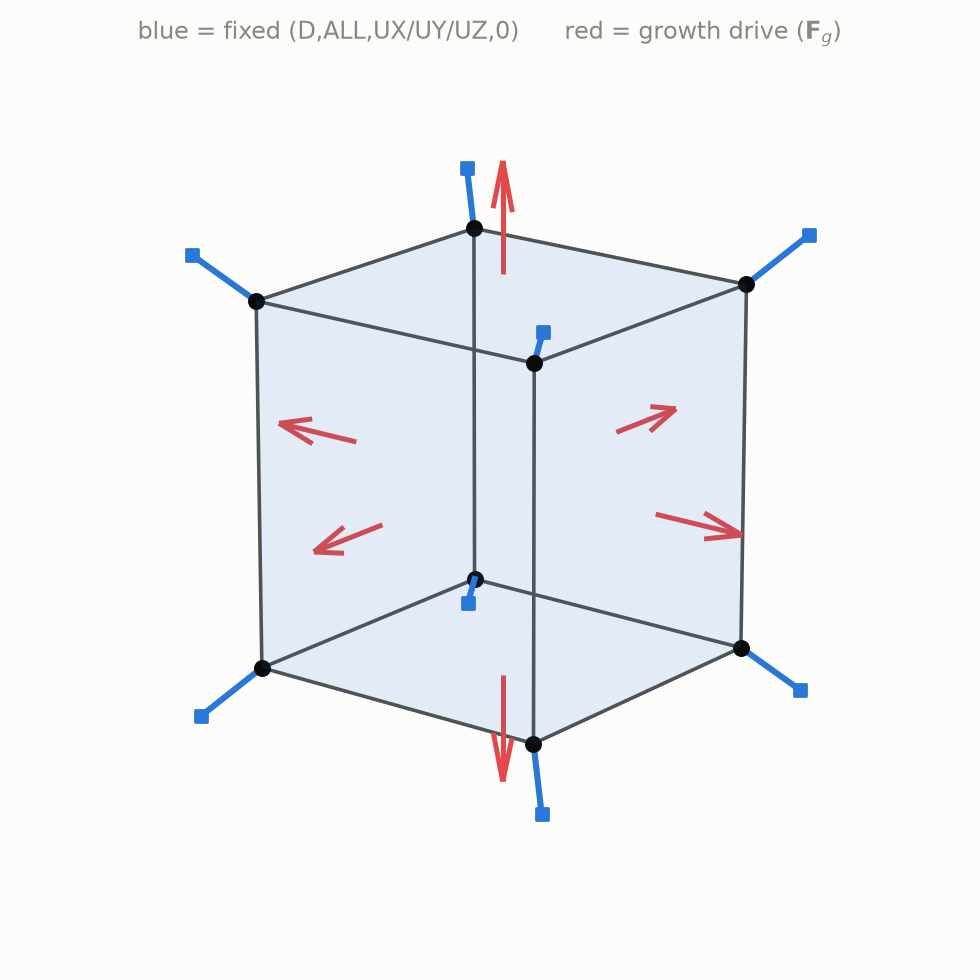
\includegraphics[width=\linewidth]{assets/growth_bc_3d.png}
\end{column}
\begin{column}{0.45\textwidth}
\small
Single \texttt{SOLID185}, unit cube, \textbf{all 8 nodes fully fixed}.
\vspace{4pt}
\begin{itemize}
  \item Constraint forces $\mathbf F=\mathbf I$ exactly at every Gauss point
        --- no FE solve needed to know the deformation
  \item $\mathbf F_g=(1{+}\alpha)\mathbf I$ makes the material want to grow
        isotropically and it can't $\Rightarrow$ pure hydrostatic compression,
        \textbf{known in closed form}
  \item The 4 cases (next slide): elastic/viscous $\times$
        $\alpha{=}0.05/0.20$ --- same cube, same BCs, different growth/viscosity
\end{itemize}
\end{column}
\end{columns}
\end{frame}

% --------------------------------------------------------
\begin{frame}{Caveat: this cube is a math check, not the biofilm's actual shape}
\small
The single constrained cube isolates the \textbf{growth law itself} --- it
says nothing about real geometry. Real oral biofilms are considerably more
structured:
\vspace{4pt}
\begin{itemize}
  \item \textbf{Mushroom/pillar + water channels} --- typical under flow
        (rivers, catheters); the textbook confocal image
  \item \textbf{Flat, layered mat} (tens--hundreds of \textmu m thick) ---
        typical of static, nutrient-rich, diffusion-limited conditions ---
        \textbf{closer to dental plaque}
  \item Tooth/implant surfaces are \textbf{curved, heterogeneous substrates},
        not flat or cubic --- early colonizers (\emph{S.\ oralis},
        \emph{A.\ naeslundii}) form a thin base layer, late pathogens
        (\emph{P.\ gingivalis}) colonize \textbf{patchily} on top
        (the composition variability CLSM measures)
  \item Gingival sulcus / peri-implant gap geometry itself constrains the
        mechanics --- not captured by a free cube
\end{itemize}
\vspace{4pt}
{\scriptsize The real geometry path (patient-specific STL/CT $\to$ conformal
mesh) is separate machinery (\texttt{biofilm\_conformal\_tet.py},
\texttt{openjaw\_*.py}) --- not run for tonight's verification.}
\end{frame}

% --------------------------------------------------------
\begin{frame}{Update: the growth branch now runs inside real ANSYS}
\textbf{Since the benchmark slide:} built the custom ANSYS 2022 R2 executable
with \texttt{usermat\_biofilm.f} linked in, and ran the closed-form
growth-branch check (element fully constrained, $\mathbf F=\mathbf I$, so
$\boldsymbol\sigma$ is known analytically --- no FE solve needed to predict it).
\vspace{2pt}
\begin{columns}[T]
\begin{column}{0.5\textwidth}
\begin{table}
\centering\scriptsize
\begin{tabular}{@{}llr@{}}
\toprule
Case & \texttt{KEYOPT} & \\
\midrule
elastic, $\alpha{=}0.05$ & 0/2/3 & \textbf{match, all 3}\\
viscous, $\alpha{=}0.05$ & 0 & \textbf{match}\\
elastic, $\alpha{=}0.20$ & 0 & \textbf{match}\\
viscous, $\alpha{=}0.20$ & 0 & \textbf{match}\\
\bottomrule
\end{tabular}
\end{table}
All 4 reference cases \emph{and} the \texttt{KEYOPT} formulation sweep
(B-bar / enhanced / simplified enhanced strain) match exactly --- no
volumetric locking on this load. First time the growth branch has run
end-to-end inside ANSYS, not just the standalone crosscheck driver.
\end{column}
\begin{column}{0.5\textwidth}
  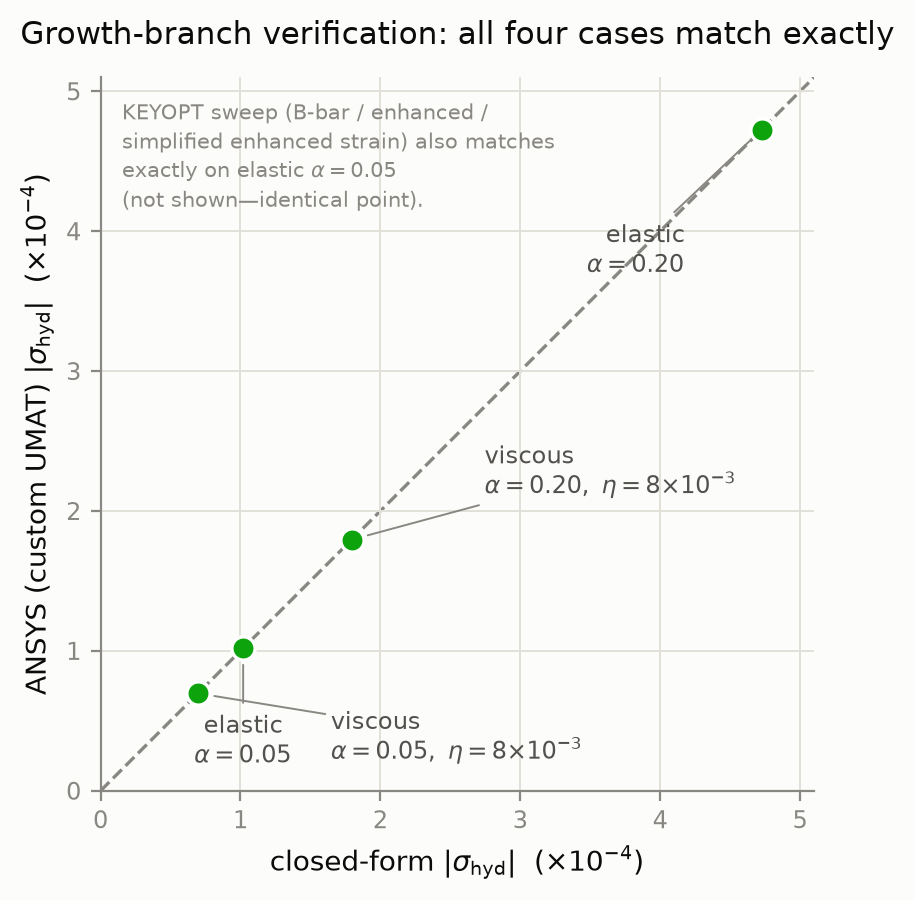
\includegraphics[width=\linewidth]{assets/growth_verify_parity.png}
\end{column}
\end{columns}
\end{frame}

% --------------------------------------------------------
\begin{frame}{Two real bugs found along the way --- both fixed}
\begin{columns}[T]
\begin{column}{0.48\textwidth}
\begin{center}
\colorbox{c3!12}{\parbox{0.95\linewidth}{\centering
\textbf{\textcolor{c3}{Bug 1 --- link error}}\\[3pt]
\footnotesize
\textbf{Symptom:} unresolved symbol\\[2pt]
\textbf{Looked like:} compiler mismatch\\[2pt]
\textbf{Actually:} 1 line missing from\\ ANSYS's own link script\\[2pt]
\textbf{Fix:} 1 line, no reinstall
}}
\end{center}
\end{column}
\begin{column}{0.48\textwidth}
\begin{center}
\colorbox{todo!10}{\parbox{0.95\linewidth}{\centering
\textbf{\textcolor{todo}{Bug 2 --- silent state bug}}\\[3pt]
\footnotesize
\textbf{Symptom:} viscous case = elastic\\ case, no crash\\[2pt]
\textbf{Cause:} \texttt{TBDATA} caps at\\ 6 values/call --- deck's 9-value\\
init silently dropped the tail\\[2pt]
\textbf{Fix:} split into 2 calls
}}
\end{center}
\end{column}
\end{columns}
\vspace{10pt}
\centering
{\scriptsize Full writeup: \texttt{ansys\_usermat/apdl/RUNBOOK.md} ---
diagnosed by instrumenting the UMAT with debug output and tracing exactly
what ANSYS passed to the material.}
\end{frame}

% --------------------------------------------------------
\begin{frame}{A second, independent closed-form check: free growth}
\small The constrained cube forces $\mathbf F=\mathbf I$ regardless of
whether $\mathbf F_g$/$\mathbf F_g^{-1}$ are wired with the right sign --- a
sign error and its inverse could in principle cancel out under that much
kinematic constraint. So: same cube, opposite extreme. Only the 6 rigid-body
modes removed, everything else traction-free --- the element is free to
actually grow.
\vspace{4pt}
\begin{center}
\begin{tabular}{@{}lll@{}}
\toprule
& Closed form & ANSYS (custom UMAT)\\
\midrule
stress & $\equiv 0$ (any $\alpha,\eta$) & $\sim\!1.9\times10^{-10}$\\
shear & $0$ & $\sim\!1.8\times10^{-14}$\\
\bottomrule
\end{tabular}
\end{center}
\vspace{4pt}
Zero to solver tolerance --- nine orders of magnitude below the constrained
case's stress scale. Two independent closed-form checks now agree, from
opposite kinematic extremes.
\end{frame}

% --------------------------------------------------------
\begin{frame}{Next: moving past the cube (in progress, not yet converged)}
\small Direct response to the caveat a few slides back --- a first attempt
at a shape closer to a tooth surface: a curved \textbf{substrate}
(no growth) bonded to a thin \textbf{growth layer} (biofilm) on top.
\vspace{4pt}
\begin{itemize}
  \item Not closed-form (two bonded curved layers have no simple analytic
        answer) --- a qualitative smoke test, not a pass/fail check
  \item Found and fixed two real input bugs on the way: \texttt{VGLUE}
        silently drops material assignment across its own volume
        renumbering; a mesh size coarser than the thin layer's own
        thickness produces degenerate elements regardless of load
  \item \textbf{Current status: does not converge yet} --- the solve hits
        element distortion independent of growth magnitude or substep
        count. Smells like a genuine bending/near-incompressibility
        difficulty with the current boundary conditions, not a leftover
        input bug, but that is not confirmed
\end{itemize}
\vspace{4pt}
{\scriptsize Parked, not abandoned: further debugging needs disk headroom
this workstation is currently short on (unrelated IT issue, being chased
separately). Deck and full diagnosis:
\texttt{ansys\_usermat/apdl/t\_growth\_cylinder\_shell.dat}.}
\end{frame}

% --------------------------------------------------------
\begin{frame}{UserElement vs.\ UserMat: narrowed, not settled}
\small The assignment says \emph{UserElement/UserMat}; this repo has a
UserMat only --- it can't transport the ecology field spatially by itself.
\vspace{6pt}
\begin{table}
\centering\small
\begin{tabular}{@{}p{4.6cm}p{4.6cm}@{}}
\toprule
\textcolor{c3}{\textbf{Carries over either way}} & \textcolor{todo}{\textbf{Genuinely new work}}\\
\midrule
Our verified UMAT, unchanged --- a UserElement can call it directly
(\texttt{KEYANSMAT=1} $\to$ \texttt{ElemGetMat}, confirmed from ANSYS's own
example) &
Field-DOF residual for the ecology transport --- \textbf{no template} in
ANSYS's own example, either way\\
\bottomrule
\end{tabular}
\end{table}
\vspace{4pt}
\centering
\colorbox{c3!12}{\parbox{0.9\linewidth}{\centering\small
\textbf{Working assumption, pending Oliver/Meisam:} extra nodal DOFs inside a
UserElement --- not precomputed externally, as this repo does today}}
\vspace{6pt}
{\scriptsize Notes: \texttt{ansys\_usermat/USERELEM\_NOTES.md}. Still waiting
on Felix's implementation from Oliver --- \texttt{crosscheck.py} is ready to
diff against it the moment it arrives.}
\end{frame}

% --------------------------------------------------------
\begin{frame}{Validation on the 2-D mesh}
\begin{itemize}
  \item Stress--strain relation checked at Gauss-point level
  \item Equilibrium $\operatorname{div}\boldsymbol{\sigma}=\mathbf{0}$:
        patch test / manufactured solution
  \item Residual convergence under mesh refinement
\end{itemize}
\vspace{4pt}
{\scriptsize \TODO{figure: FEM residual convergence plot --- pending}}
\end{frame}

% --------------------------------------------------------
\begin{frame}{Species count: keeping the full 5-species model}
\begin{itemize}
  \item Full model: 5 oral species (\emph{S.\ oralis}, \emph{A.\ naeslundii},
        \emph{Veillonella}, \emph{F.\ nucleatum}, \emph{P.\ gingivalis}) --- early
        colonizers through the late pathogen
  \item Decision: \textbf{no reduction} --- keep all 5 inside the Gauss-point
        loop; the UMAT coupling (route 3) keeps the per-call cost low enough
        that a cut is not needed
  \item Outlook: scale back up further (100+ species, clinical metagenomes)
        once the coupling is efficient
\end{itemize}
\end{frame}

% --------------------------------------------------------
\begin{frame}{Timeline to submission}
\centering
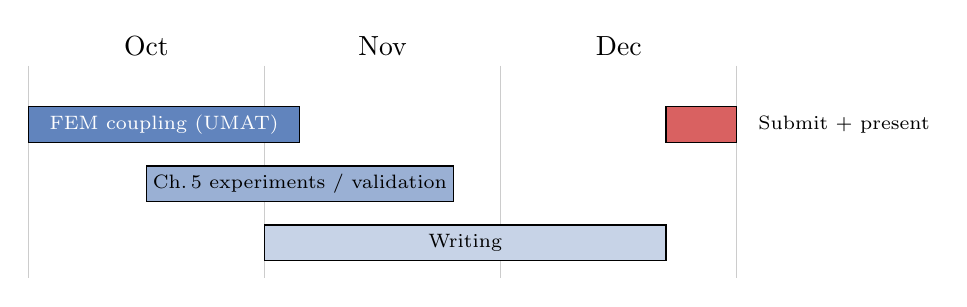
\begin{tikzpicture}[x=3.0cm, y=-0.75cm]
  % month gridlines
  \foreach \m/\lbl in {0/Oct, 1/Nov, 2/Dec} {
    \draw[gray!40] (\m,0) -- (\m,3.6);
    \node[above] at (\m+0.5,0) {\lbl};
  }
  \draw[gray!40] (3,0) -- (3,3.6);
  % row 1: UMAT/FEM coupling
  \draw[fill=c3!70] (0,0.7) rectangle (1.15,1.3);
  \node[white,font=\scriptsize] at (0.575,1.0) {FEM coupling (UMAT)};
  % row 2: ch.5 experiments / validation
  \draw[fill=c3!45] (0.5,1.7) rectangle (1.8,2.3);
  \node[font=\scriptsize] at (1.15,2.0) {Ch.\,5 experiments / validation};
  % row 3: writing
  \draw[fill=c3!25] (1.0,2.7) rectangle (2.7,3.3);
  \node[font=\scriptsize] at (1.85,3.0) {Writing};
  % row 4: submit + present
  \draw[fill=todo!70] (2.7,0.7) rectangle (3.0,1.3);
  \node[font=\scriptsize,anchor=west] at (3.05,1.0) {Submit + present};
\end{tikzpicture}
\vspace{6pt}
\begin{itemize}
  \item Submission: early--mid December (before returning to Japan)
  \item Presentation: December, date to be fixed with both examiners
  \item Keio side: credit transfer / DD paperwork \TODO{ask Prof.\ Muramatsu}
\end{itemize}
\end{frame}

% --------------------------------------------------------
\begin{frame}{Questions for this meeting}
\begin{enumerate}
  \item Keio: anything needed from the Keio side for the DD requirements this term?
  \item UserElement vs.\ UserMat: does the working assumption on the previous
        slide look right, or is there a reason to prefer the other route?
  \item Presentation: online attendance from Japan possible for Prof.\ Muramatsu?
\end{enumerate}
\end{frame}

\end{document}